\pagestyle{empty}

\begin{appendices}
    \appendixheaderon
    \singlespacing

    \section{Structure du code}
    \begin{figure}[H]
        \centering
        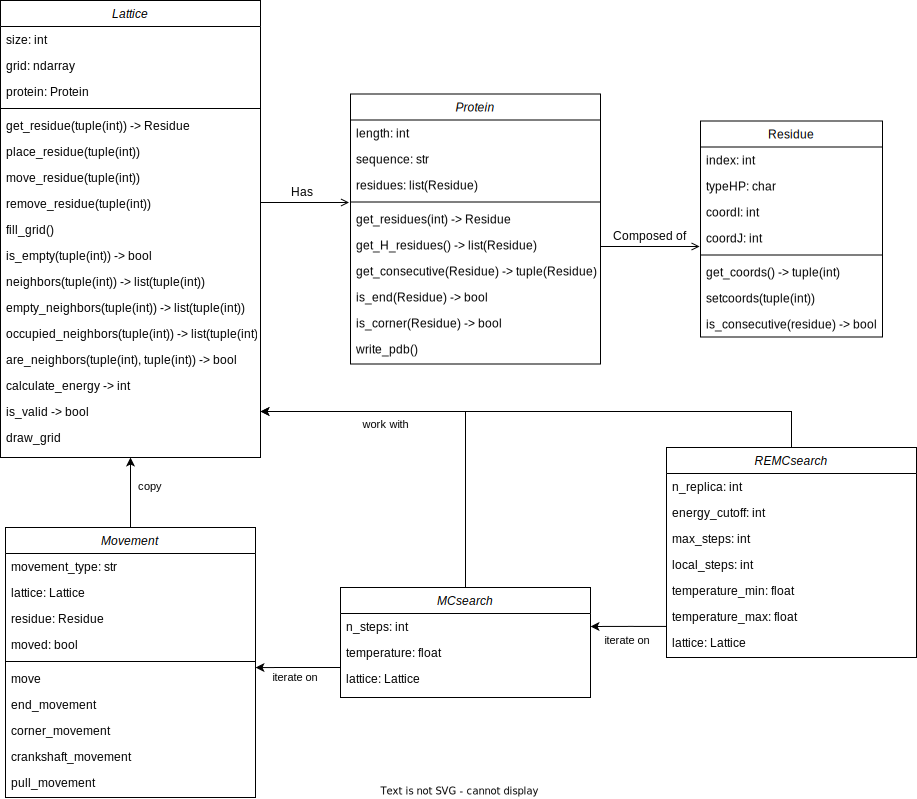
\includegraphics[width=\textwidth]{figures/class_dependencies.png}
        \caption{Structure des classes et fonctions principales}
        \label{fig:class_dependencies}
    \end{figure}

    \section{Sorties des runs de benchmarking}
    \begin{verbatim}
Running test case: HPHPPHHPHPPHPHHPPHPH with optimal energy: -9
Running MC with parameters: n-steps=5000, temperature=200
Final lattice with energy of -4
+-----------+
|           |
|        PP |
| PH     HH |
| HHHPHHPHP |
| PP  PP  H |
|           |
+-----------+
Running REMC with parameters: n-replica=5, energy-cutoff=-9, max-steps=1000, local-steps=100, temperature-min=160, temperature-max=220
Final lattice with energy of -4
+--------------+
|              |
| PH        PP |
| HHHPHPPHPHHH |
| PP        HP |
|              |
+--------------+
\end{verbatim}

\begin{verbatim}
Running test case: HHPPHPPHPPHPPHPPHPPHPPHH with optimal energy: -9
Running MC with parameters: n-steps=5000, temperature=200
Final lattice with energy of -4
+------------------+
|                  |
|             PPHP |
| HHPPHPPHHPPHHHHP |
|        PP  PP    |
|                  |
+------------------+
Running REMC with parameters: n-replica=5, energy-cutoff=-9, max-steps=500, local-steps=100, temperature-min=160, temperature-max=220
Final lattice with energy of -3
+-------------------+
|                   |
| HPP           PP  |
| HHHPPHPPHPPHPPHHH |
| PP                |
|                   |
+-------------------+
\end{verbatim}

\begin{verbatim}
Running test case: PPHPPHHPPPPHHPPPPHHPPPPHH with optimal energy: -8
Running MC with parameters: n-steps=5000, temperature=200
Final lattice with energy of -3
+---------+
|         |
|  PP     |
| PPP PH  |
| PHH PHP |
| HHHPPPP |
| PP   P  |
|     HH  |
|         |
+---------+
Running REMC with parameters: n-replica=5, energy-cutoff=-8, max-steps=500, local-steps=100, temperature-min=160, temperature-max=220
Final lattice with energy of -1
+----------------------+
|                      |
| PP               PHH |
| HHHPPPPHHPPPPHHPPP   |
| P                    |
| P                    |
|                      |
+----------------------+
\end{verbatim}

\end{appendices}